\documentclass[18 pt]{beamer}
\usetheme{Madrid}
% \usefonttheme{professionalfonts}
\usefonttheme{structurebold}
\usecolortheme{rose}
\setbeamerfont{title}{size=\LARGE, series=\bfseries}
% \setbeamerfont{subtitle}{size=\large}
% \setbeamerfont{author}{size=\large}
% \setbeamerfont{date}{size=\large}
% \setbeamerfont{frametitle}{size=\Large, series=\bfseries}
% \setbeamerfont{framesubtitle}{size=\large}
% \setbeamerfont{normal text}{size=\huge}
\usepackage{enumitem}
\setlist[enumerate]{label=\arabic*)., leftmargin=*,itemsep=30pt}
\setbeamerfont{enumerate item}{size=\LARGE}
\setlist[itemize]{label=\textbullet, leftmargin=*, itemsep=5pt}

\usepackage{amsmath}
\usepackage{amssymb}
\usepackage{listings}
\usepackage{booktabs}
\usepackage{multirow}
\usepackage{multirow}
\usepackage{lmodern}
\usepackage{xcolor}
\usepackage{float}
\lstset{
  language=Python,  %代码语言使用的是matlab
  % frame=shadowbox, %把代码用带有阴影的框圈起来
  rulesepcolor=\color{red!20!green!20!blue!20},%代码块边框为淡青色
  keywordstyle=\color{blue!90}\bfseries, %代码关键字的颜色为蓝色,粗体
  commentstyle=\color{red!10!green!70}\textit,    % 设置代码注释的颜色
  basicstyle=\footnotesize,
  showstringspaces=true,%不显示代码字符串中间的空格标记
  % numbers=left, % 显示行号
  % numberstyle=8pt,    % 行号字体
  % numberstyle=\color{green},
  stringstyle=\rmfamily\slshape\color[RGB]{128,0,0}, % 代码字符串的特殊格式
  breaklines=true, %对过长的代码自动换行
  extendedchars=false,  %解决代码跨页时,章节标题,页眉等汉字不显示的问题
  escapeinside=``,%代码中出现中文必须加上,否则报错
  texcl=true}

\lstset{breaklines}%自动将长的代码行换行排版

\lstset{extendedchars=false}%解决代码跨页时,章节标题,页眉等汉字不显示的问题

\usepackage{textcomp}
% \usepackage[margin=1in]{geometry}
\usepackage{pythonhighlight}
% \usepackage{minted}
\usepackage[backend=bibtex]{biblatex}
%\usepackage[style=authortitle,backend=biber]{biblatex}
\addbibresource{ResearchRabbit_Export_2022_10_20.bib}

\usepackage{algorithm}
\usepackage{algorithmic}
\renewcommand{\algorithmicrequire}{\textbf{Input:}}
\renewcommand{\algorithmicensure}{\textbf{Output:}}

% //TODO: add
\AtBeginSection[]{
  \begin{frame}
  \frametitle{Outline}
  \tableofcontents[currentsection,hideallsubsections]
  \end{frame}
}
\AtBeginSubsection[]{
  \begin{frame}
  \frametitle{Outline}
  \tableofcontents[currentsubsection]
  \end{frame}
}
\setbeamertemplate{section in toc}{\inserttocsectionnumber.~\inserttocsection}
\setbeamertemplate{subsection in toc}[ball unnumbered]
\setbeamertemplate{subsubsection in toc}[square unnumbered]


\title{Synthesis on Atom Computation}
\author[Gcc]{Dingchao Gao}
\institute[ISCAS]{Institute of Software Chinese Academy of Sciences}

\setbeamertemplate{footline}[frame number]
\begin{document}
\begin{frame}[plain]
    \titlepage
  \end{frame}
% \begin{frame}
%     \frametitle{Outline}
%     \begin{itemize}
%         \item Quick review
%         \item Paper call back
%         \item Discussion
%     \end{itemize}
% \end{frame}

\begin{frame}
    \frametitle{Quick Review}
    \begin{itemize}
        \item Neutral atom controlled by laser lattice (stationary) and laser tweezers (move)
        \item Single qubit gate $U3: (\Omega\tau\cos{\varphi},\Omega\tau\sin{\varphi},\delta\tau)$
        \item Multi-qubit gate $C\mathcal{Z}: 2|gg\rangle\langle gg| - I$
    \end{itemize}
\end{frame}

\begin{frame}
    \frametitle{Paper Call Back}
    \begin{itemize}
        \item Setup (the constraints it considered)
        \item Optimize goal (the cost it wants to reduce)
        \item Methods (how it finishes)
    \end{itemize}
\end{frame}
\section{Decomposing and Routing Quantum Circuits Under Constraints for Neutral Atom Architectures}

\begin{frame}
    \frametitle{Setup}
    \begin{itemize}
        \item \textit{StandardGateSet}: $\{U_3,CZ\}$
        \item Existing hardware does not support local addressing for all qubit rotations:
        \begin{itemize}
            \item Local $CZ$
            \item Local $R_Z(\lambda), (0,0,\frac{\lambda}{2})$
            \item Global $GR(\theta,\phi), (\frac{\theta}{2}\cos{\phi},\frac{\theta}{2}\sin{\phi},0)$
        \end{itemize}
        \item Atom movement
    \end{itemize}
\end{frame}

\begin{frame}
    \frametitle{Optimization Goal}
    The primary optimization goal is to minimize:
    \begin{itemize}
        \item Circuit duration 
        % increase overall fidelity using atom movement for better routing efficiency %
    \end{itemize}
\end{frame}

\begin{frame}
    \frametitle{Methods, \textbf{Decomposition Techniques}}
    $U3(\theta,\phi,\lambda)= RZ(\phi)RY(\theta)RZ(\lambda)$:
    \begin{itemize}
        \item $RY(\theta)= GR(\frac{-\pi}{2},0)RZ(\theta)GR(\frac{\pi}{2},0)$
        \item $RY(\theta) = Rv(\pi,\frac{\theta}{2})RZ(-\pi)$
        \item $Rv(\xi,\omega)=GR(\omega,\frac{\pi}{2})RZ(\xi)GR(-\omega,\frac{\pi}{2})$
    \end{itemize}
\end{frame}

\begin{frame}
    \frametitle{Methods, \textbf{Routing Algorithms}}
    \begin{itemize}
        \item Map
    \end{itemize}
\end{frame}

% \begin{frame}
%     \frametitle{Compiling Quantum Circuits for Dynamically Field-Programmable Neutral Atoms Array Processors}
% \end{frame}

% \begin{frame}
%     \frametitle{FPQA-C: A Compilation Framework for Field Programmable Qubit Array}
% \end{frame}
\section{Compiling Quantum Circuits for Dynamically Field-Programmable Neutral Atoms Array Processors\\FPQA-C: A Compilation Framework for Field Programmable Qubit Array}
\begin{frame}
    \frametitle{Setup (FPQA)}
    \begin{itemize}
        \item Gateset:
        \begin{itemize}
            \item Global $CZ$
            \item Local $U3$
        \end{itemize}
        \item Optical traps are configured in 2D arrays.
        \item Two-qubit entangling gates require qubits to be within a certain proximity without interfering with others.
        \item Constraints of physical movement of traps, ensuring each solution step complies with the DPQA constraints and remains executable.
    \end{itemize}
\end{frame}

\begin{frame}
    \frametitle{Constraints in the Greedy Method}
    \begin{itemize}
        \item \textbf{DPQA Architectural Constraints}:
        \begin{itemize}
            \item Adhere to movement and interaction rules specific to DPQA.
            \item Maintain the logical sequence of gate operations.
        \end{itemize}
        \item \textbf{Minimum Gates Threshold ('M')}:
        \begin{itemize}
            \item Strive to achieve at least 'M' gates per stage, where 'M' is dynamically adjusted based on solvability.
        \end{itemize}
        \item \textbf{SMT Solver Integration}:
        \begin{itemize}
            \item Use an SMT solver to find feasible solutions that maximize gate execution while respecting the constraints.
        \end{itemize}
    \end{itemize}
\end{frame}

\begin{frame}
    \frametitle{SMT Solver Role in the Greedy Method}
    \begin{itemize}
        \item \textbf{Input}: Reduced and simplified problem instances as the complexity is peeled off.
        \item \textbf{Output}: Feasible configurations that allow the maximum number of gates ('M') to be executed per stage.
        \item \textbf{Dynamic Adjustment}: Modifies 'M' based on the ease or difficulty of finding a solution, optimizing the balance between speed and completeness of the solution.
    \end{itemize}
\end{frame}

\begin{frame}
    \frametitle{Transition to Optimal Compilation}
    \begin{itemize}
        \item \textbf{Criterion for Transition}: Shifts to the optimal SMT-based approach when a significant portion of the problem has been resolved or when only a small percentage of gates remains.
        \item \textbf{Rationale}: Ensures that the final solution is both efficient and adheres strictly to all operational constraints.
    \end{itemize}
\end{frame}

\begin{frame}
    \frametitle{Conclusion}
    The integration of the SMT solver within the Greedy Method in this hybrid approach allows for a pragmatic reduction of quantum circuit complexity, setting the stage for a detailed and optimal final compilation using SMT.
\end{frame}

\begin{frame}
    \frametitle{Methods (FPQA)}
    \begin{itemize}
        \item Qubit-Array Mapper:
        \begin{itemize}
            \item K-cut problem aiming to maximize the summation of edge weights crossing different partitions
        \end{itemize}
        \item Qubit-Atom Mapper:
        \begin{itemize}
            \item SLM Array: Load balance mapping
            \item AOD Array: Alignment AOD mapping
        \end{itemize}
        \item High-Parallelism Router:
        \begin{itemize}
            \item U3 gate
            \item Check constraint
        \end{itemize}
    \end{itemize}
\end{frame}
\section{Discussion}
\begin{frame}
    \frametitle{Discussion}
    \begin{itemize}
        \item 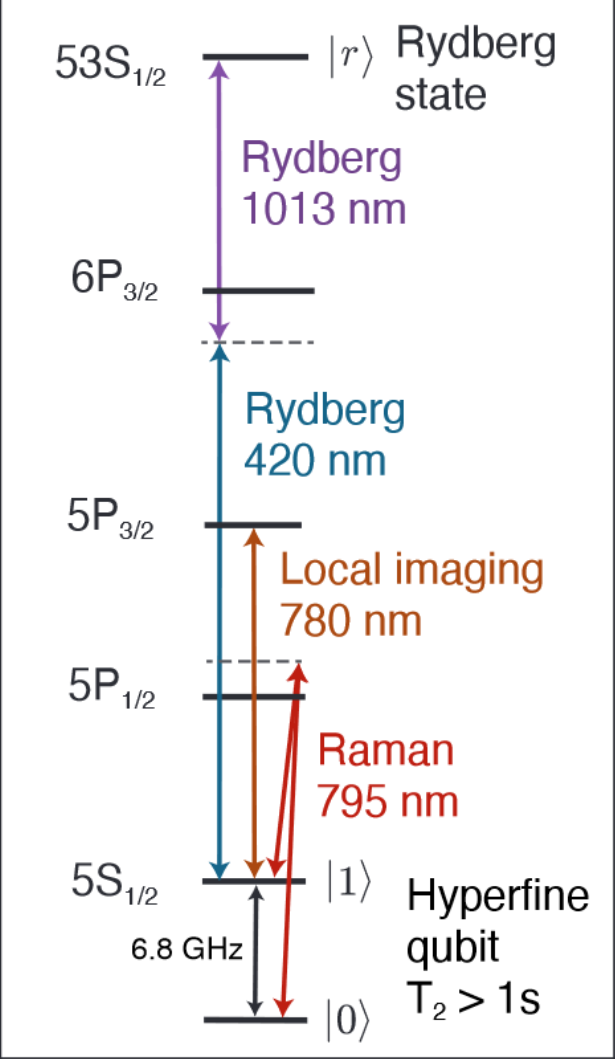
\includegraphics[width=\textwidth]{level.png}
        \item More flexible U3 gate decomposition
        \item Oracle design using z group gate
    \end{itemize}
\end{frame}

\end{document}
